\clearpage
\chapter{Results}\label{sec:results}
%Unblinded result data no excess over the standard model prediction.
CMS analyses use the ``Higgs Analysis'' group's ``Combined Limit to set limit values on various BSM processes.
The tool comes with various statistical options developed by statisticians and physicists.
We use the Combined Tool's ``AsymptoticLimits'' Approach to set limit on the branching ratio of \textbf{B}(\PH$\to SS \to \tau^{+}\tau^{-}\tau^{+}\tau^{-}$).
Assuming data events are in agreement with the SM expectation, we calculated the expected values on the exclusion limit for the branching ratio of \textbf{B}(\PH$\to SS \to \tau^{+}\tau^{-}\tau^{+}\tau^{-}$).
We input the expected background yield (B*C/D) for our factual background to calculate the expected limit values.
After calculating the expected limit, we unblind ourselves and look at the actual data event in the SR(A).
There are nine events in SR(A), which is within the statistical uncertainty of the SM expectation.
Thus, we did not find the BSM LLPs in our data from the analysis strategy.
%We use the Combined Tool again to calculate the observed limit values, where we input the actual SR(A)'s data event.
\begin{table}[htb]
\caption{Final Data entry in each region}
\begin{center}
\begin{tabular}{r|l|l}\hline
	Region & Entry & Uncertainty \\
 \hline
	CR(D) & 2151 & $\pm$ 46.37 \\
 \hline
	CR(C) & 311 & $\pm$ 17.63\\
 \hline
	CR(B) & 45 & $\pm$ 6.708\\
 \hline
	SR(B*C/D) & 6.506 & $\pm$ 2.551\\
 \hline
	SR(A) & 9 & $\pm$ 3 \\
 \hline
\end{tabular}
\label{tab:unblind}
\end{center}
\end{table}

The limits are calculated for LLP's all MS and c$\uptau$ combinations.
The best performance is observed for 15\GeV and 10mm point.
The table shows each combination's exclusion limit for 95\% confidence level (CL).
The results show significant improvement from previous tracker analysis \cite{ZHAN}.
The values are one of the most stringent results from the LHC results.

\begin{table}[htb]
\centering
\begin{tabular}{|p{3cm}|p{1cm}|p{1cm}|p{1cm}|p{1cm}|}
\hline
Lifetime & MS7 & MS15&MS40&MS55 \\
\hline
1mm & N/A & 184.4 & 65.9 & 184.4   \\
\hline
10mm & 0.0934 & 0.0402 & 0.5984 & 2.006  \\
\hline
100mm & 0.3359& 0.0514 & 0.0484 & 0.1742 \\
\hline
1000mm & 63.50 & 35.50 & 1.650  & 1.468   \\
\hline
\end{tabular}
\label{tab:Median Limit}
\centering
\caption{Median value of 95\% CL exclusion limit on the branching ratio \textbf{B}(\PH$\to SS \to \tau^{+}\tau^{-}\tau^{+}\tau^{-} $) }
\end{table}


% \begin{figure}[h!]
%   \caption{Cutflow histogram of MS15GeV-ct10mm point. Left plot is for region A, whereas the right plot is for region D}
%   \label{fig:ABmethod}
%   \centering
%   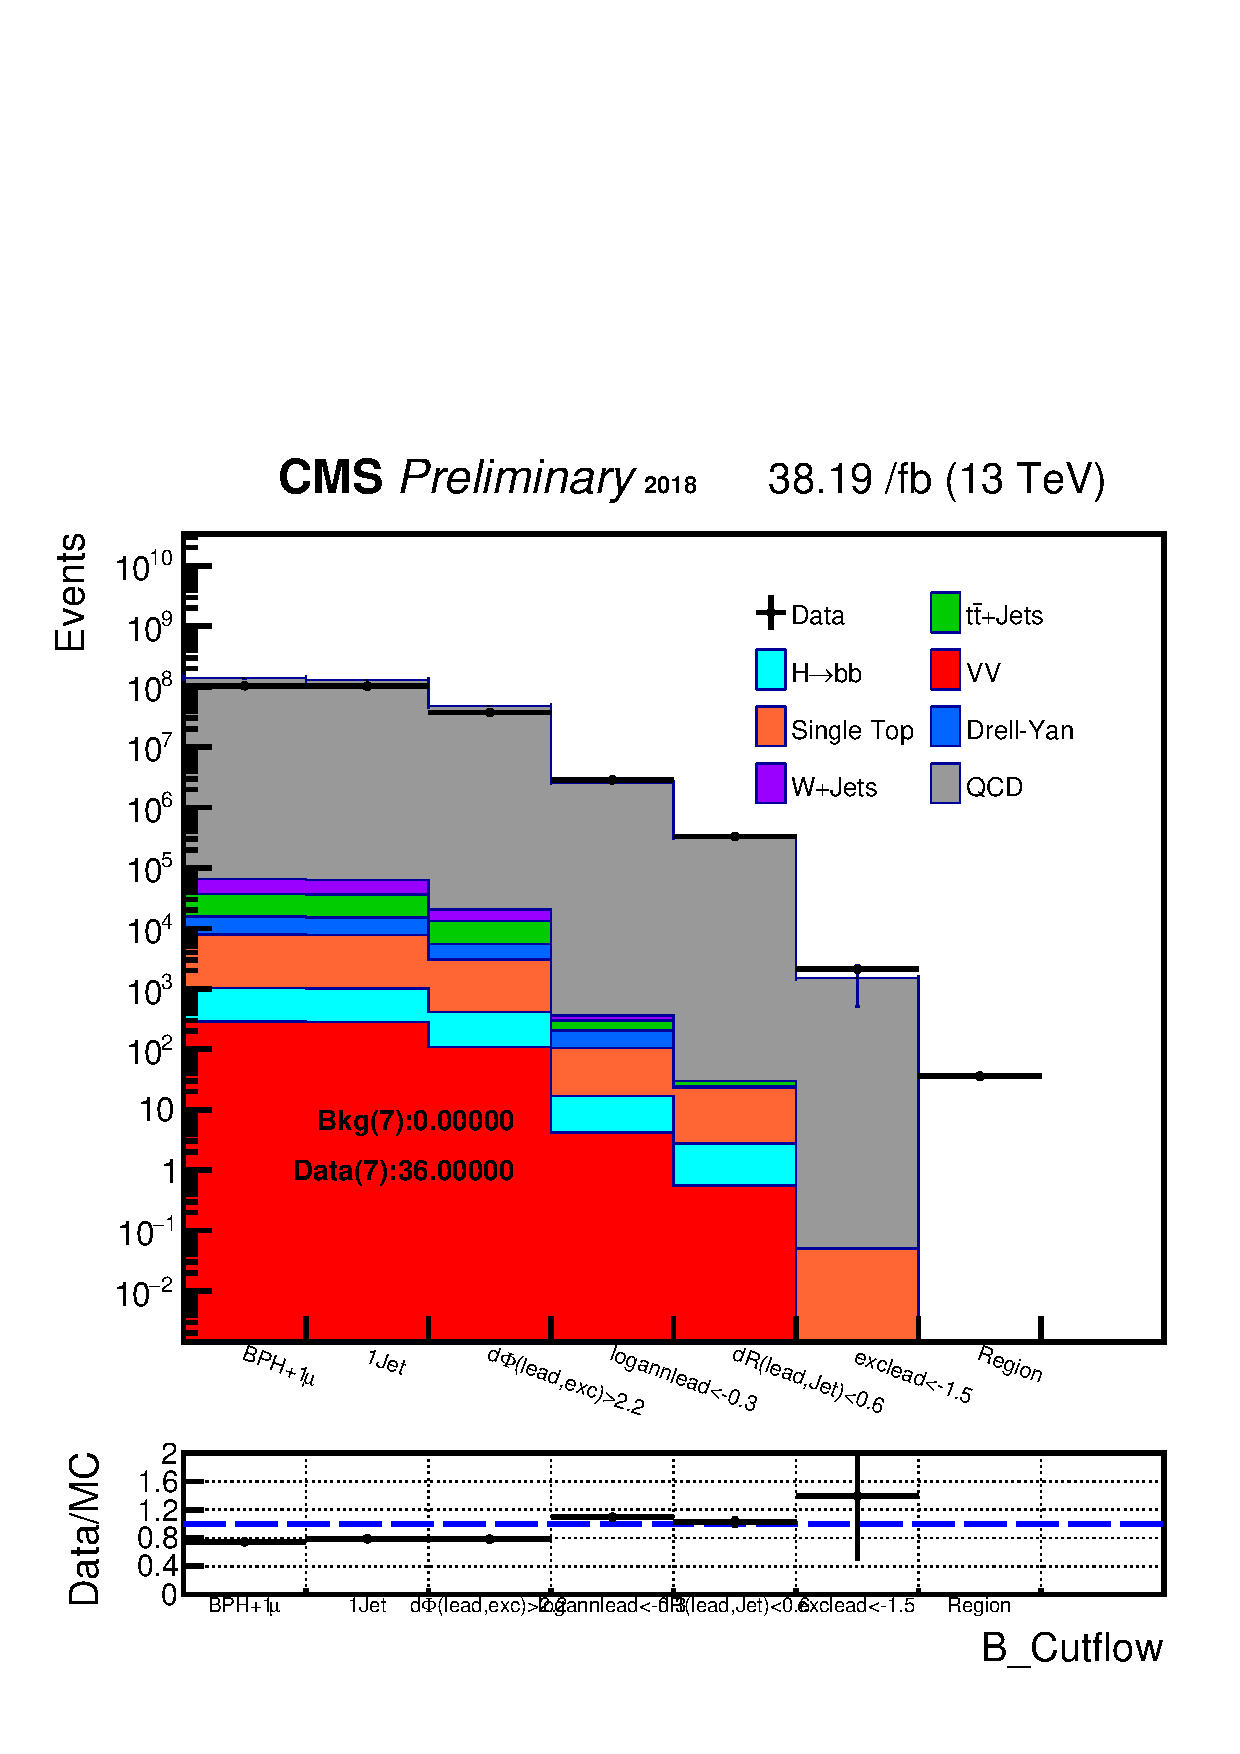
\includegraphics[width=0.47\linewidth]{figs/Data_log_CutflAnalysisNote_MS-15_ctauS-10_B_Cutflow.pdf}
%   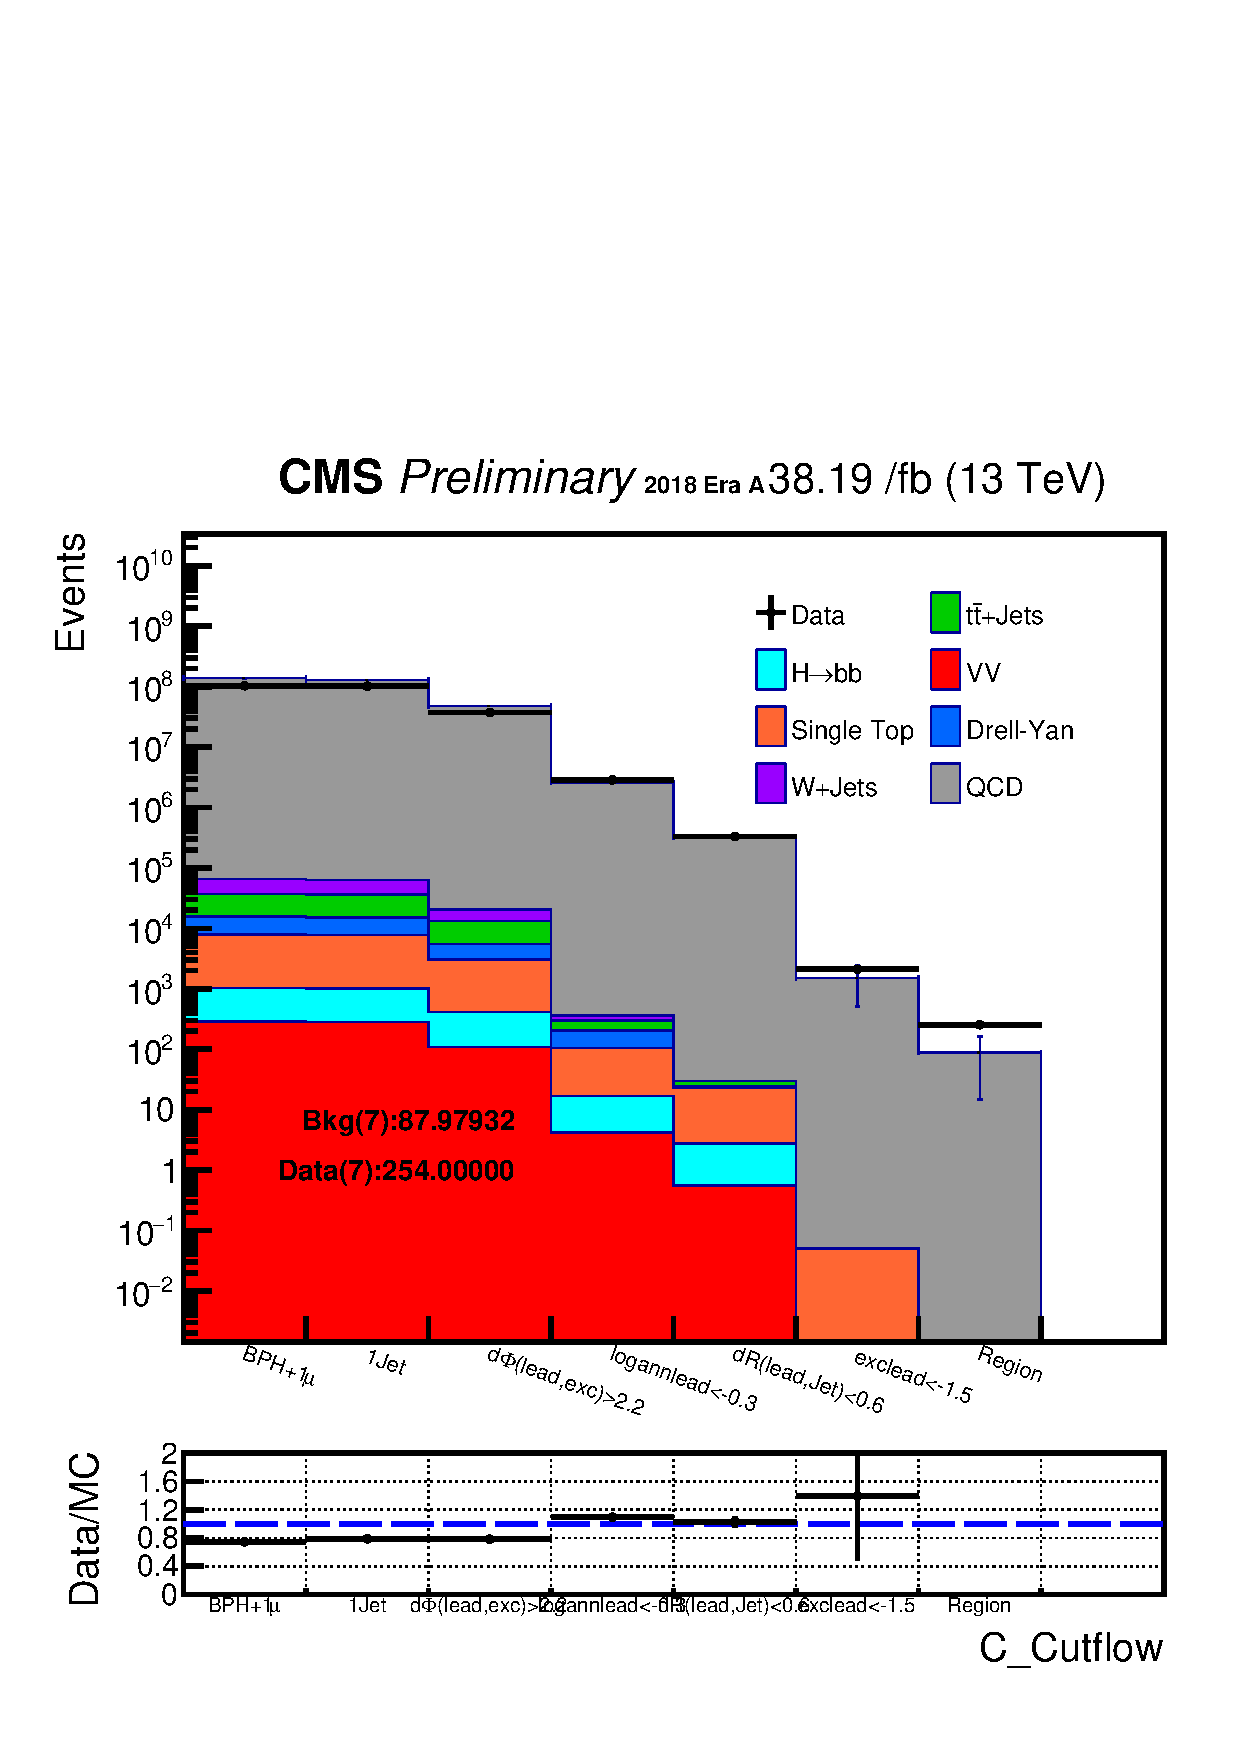
\includegraphics[width=0.47\linewidth]{figs/Data_log_CutflAnalysisNote_MS-15_ctauS-10_C_Cutflow.pdf}
%   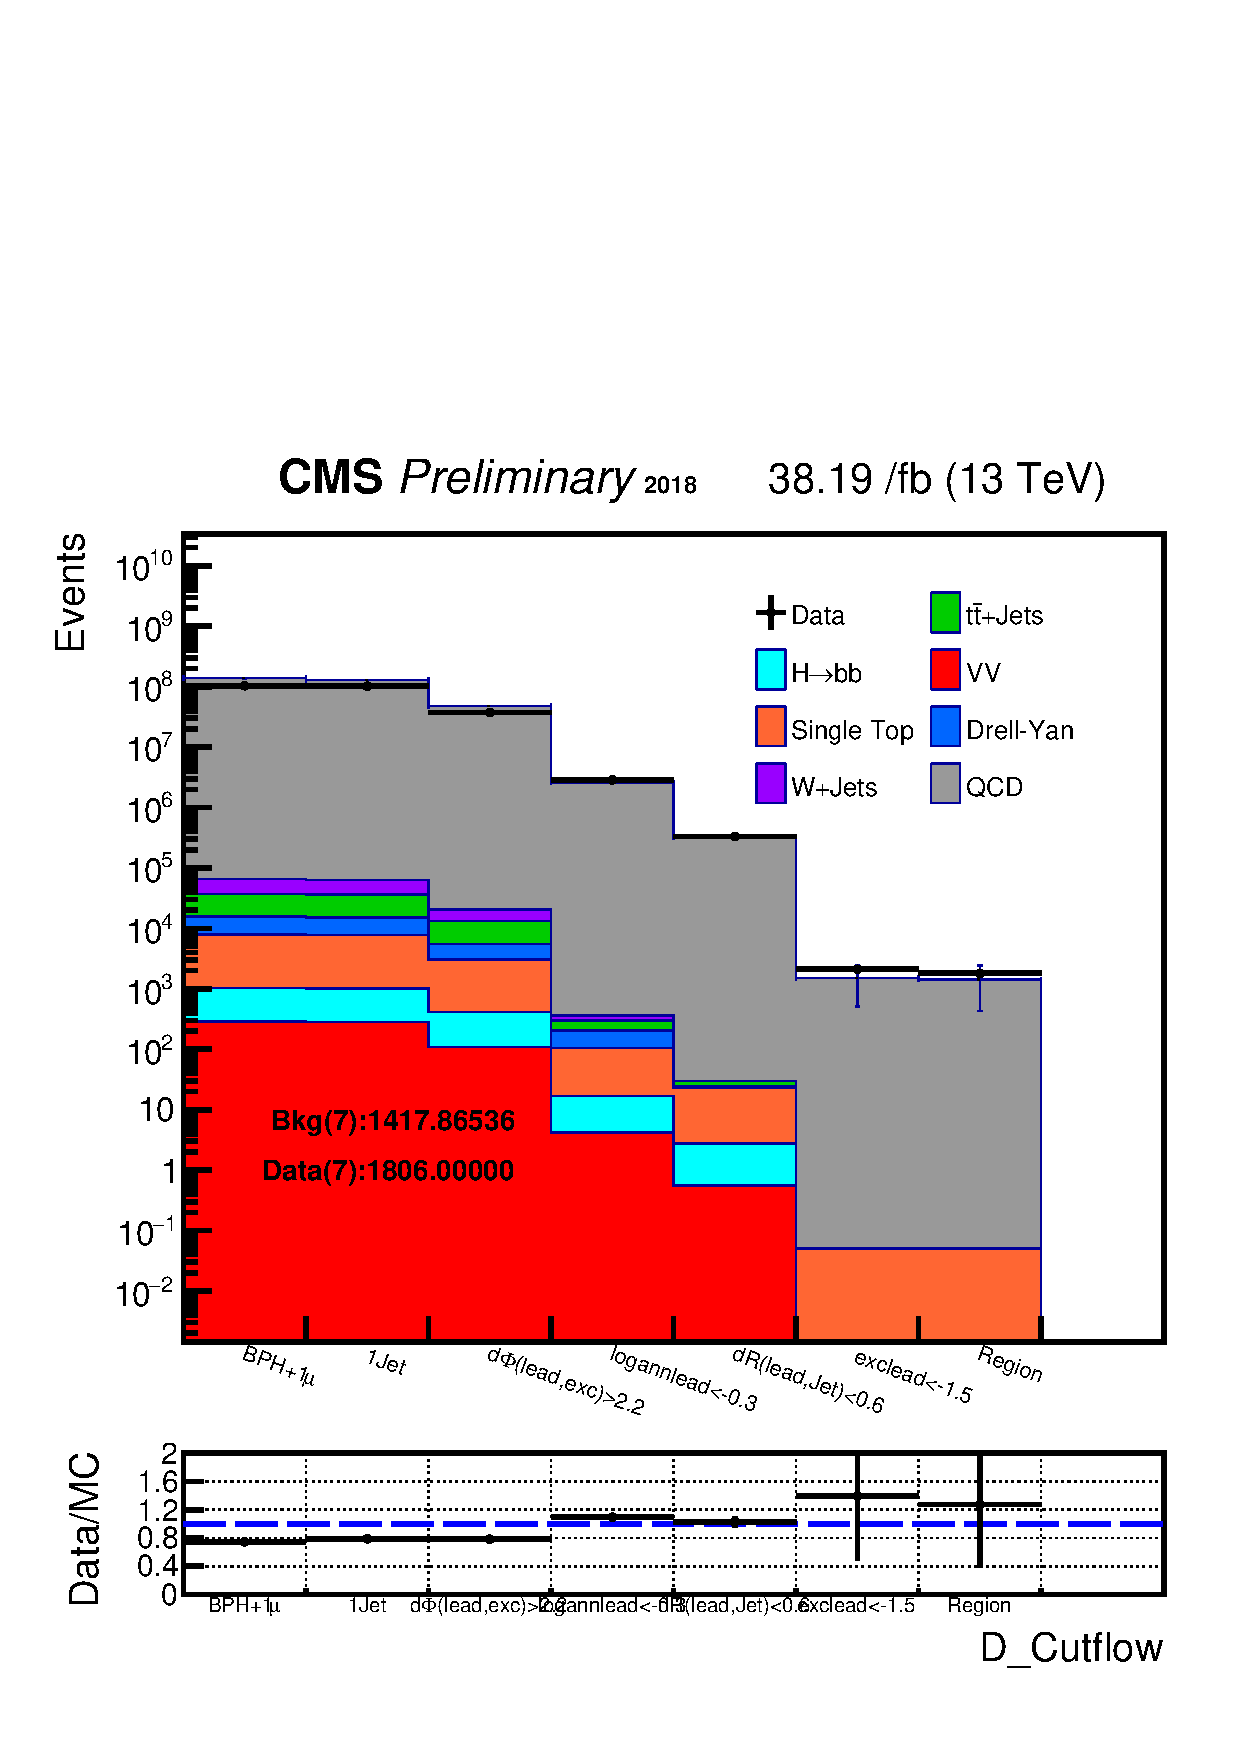
\includegraphics[width=0.47\linewidth]{figs/Data_log_CutflAnalysisNote_MS-15_ctauS-10_D_Cutflow.pdf}
% \end{figure}


\begin{figure}[h!]
   \caption{Current Preliminary limit plots for lower mass LLP}
   \label{fig:Limit}
   \centering
   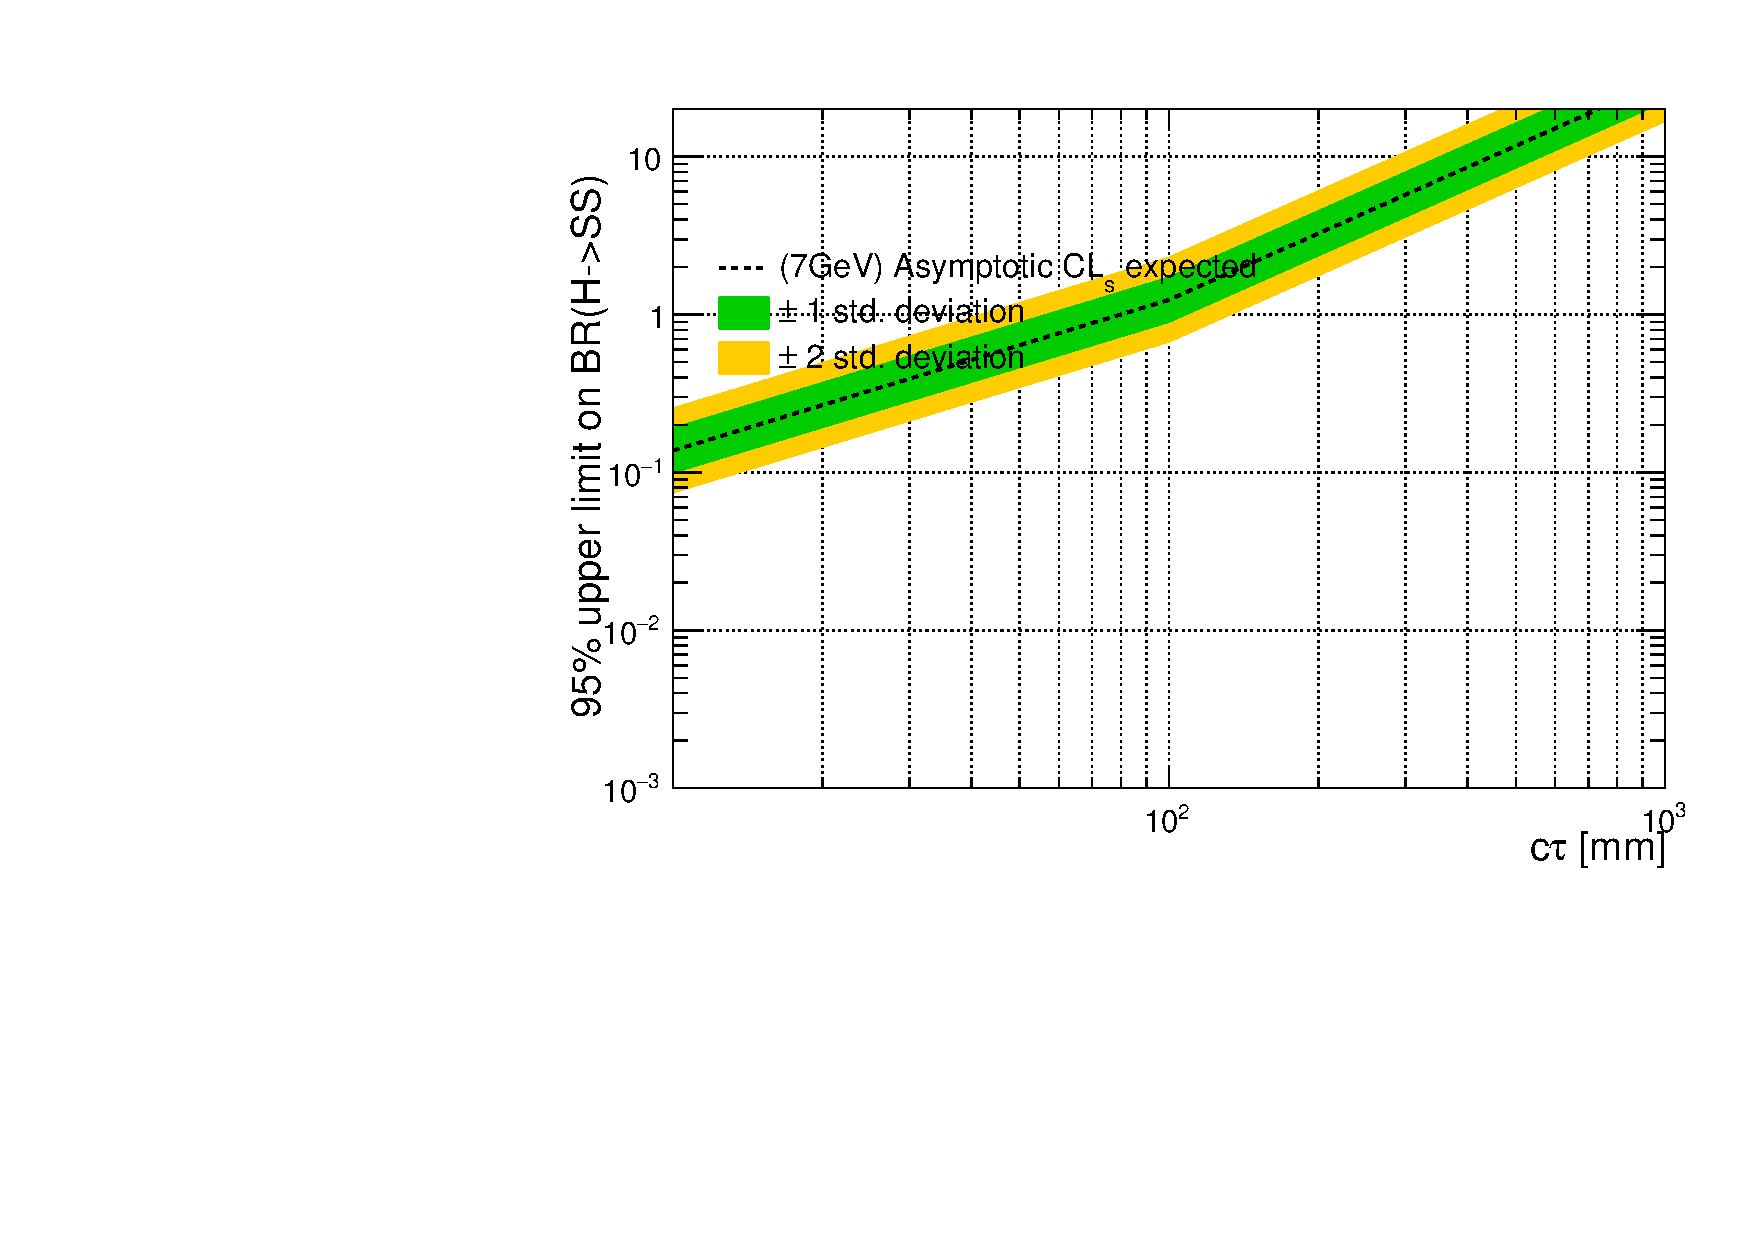
\includegraphics[width=0.48\linewidth]{figs/7GeVUpperLimit.pdf}
   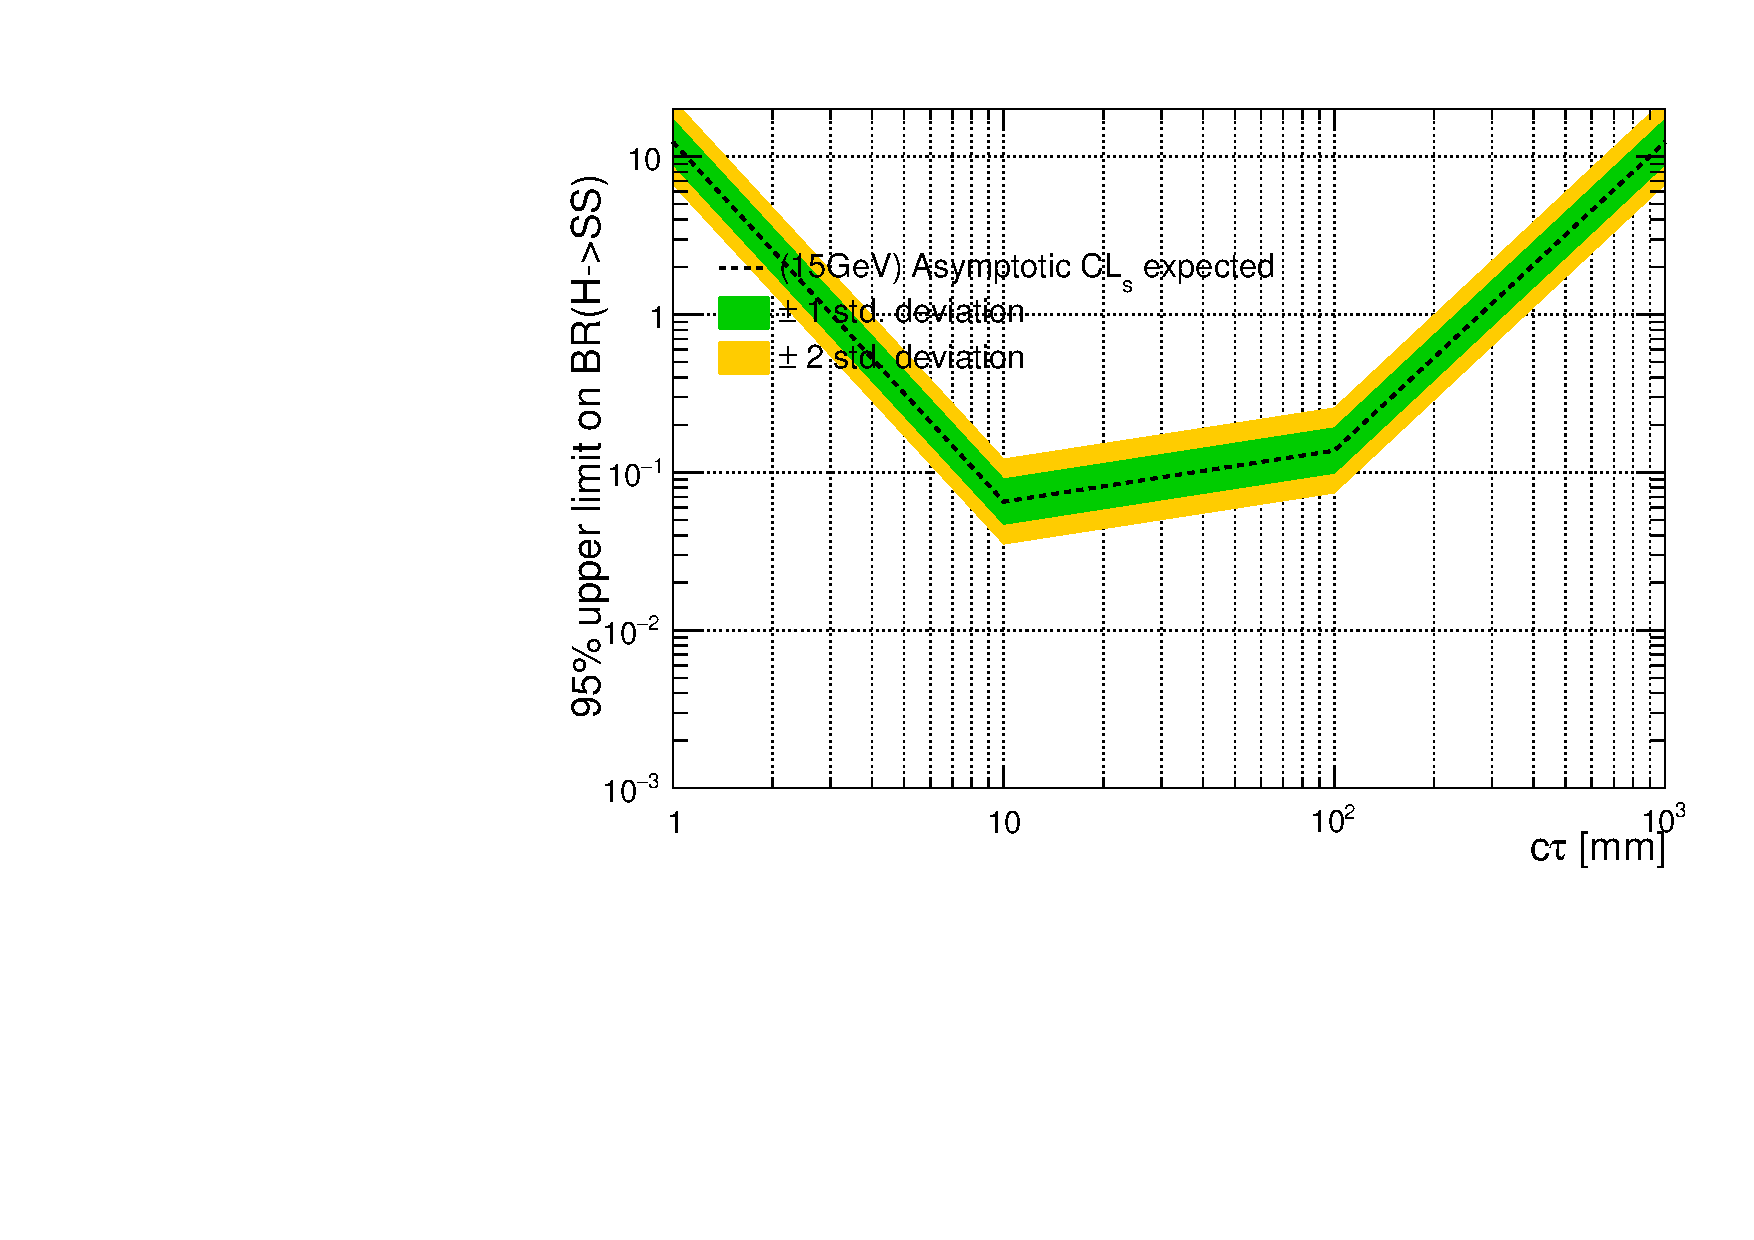
\includegraphics[width=0.48\linewidth]{figs/15GeVUpperLimit.pdf}
 \end{figure}
 \begin{figure}[h!]
   \caption{Current Preliminary limit plots for higher mass LLP}
   \label{fig:Limit2}
   \centering
   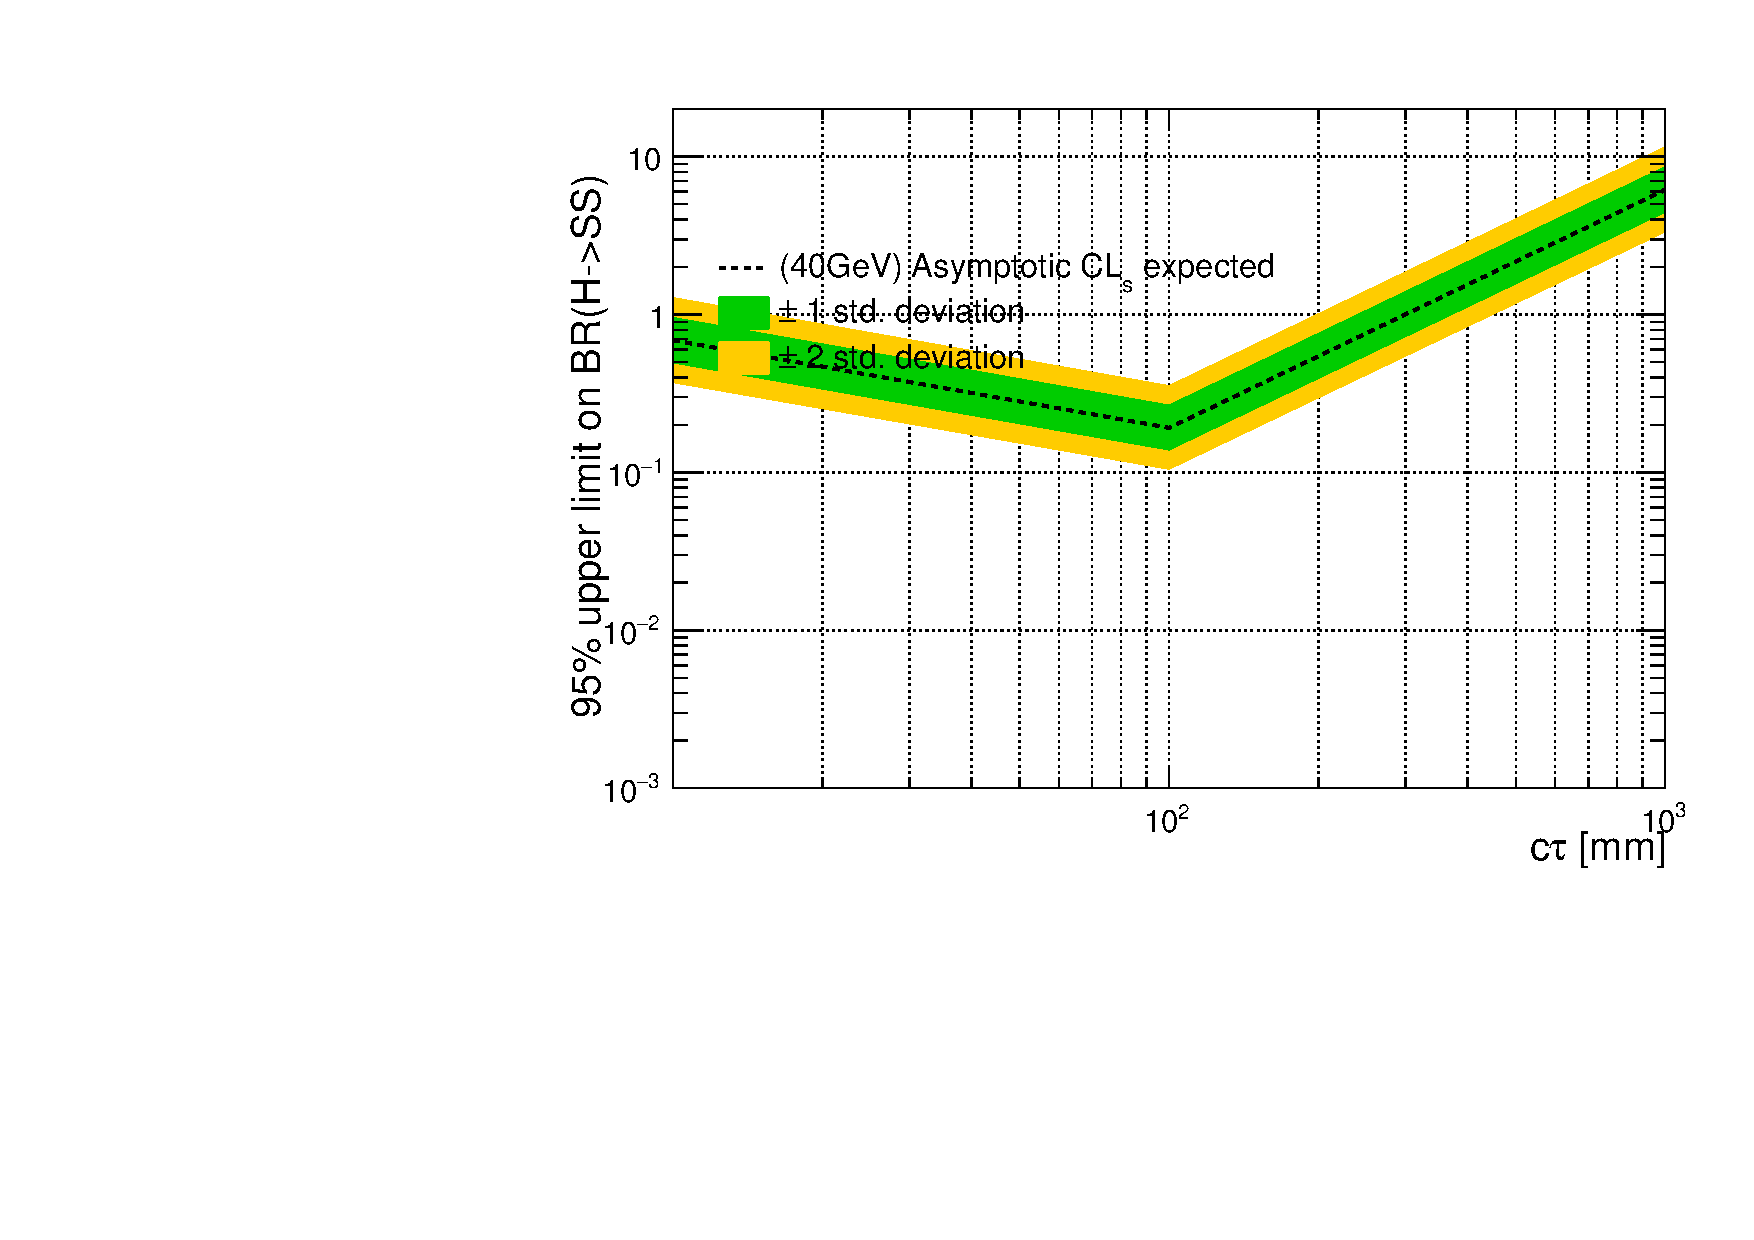
\includegraphics[width=0.48\linewidth]{figs/40GeVUpperLimit.pdf}
   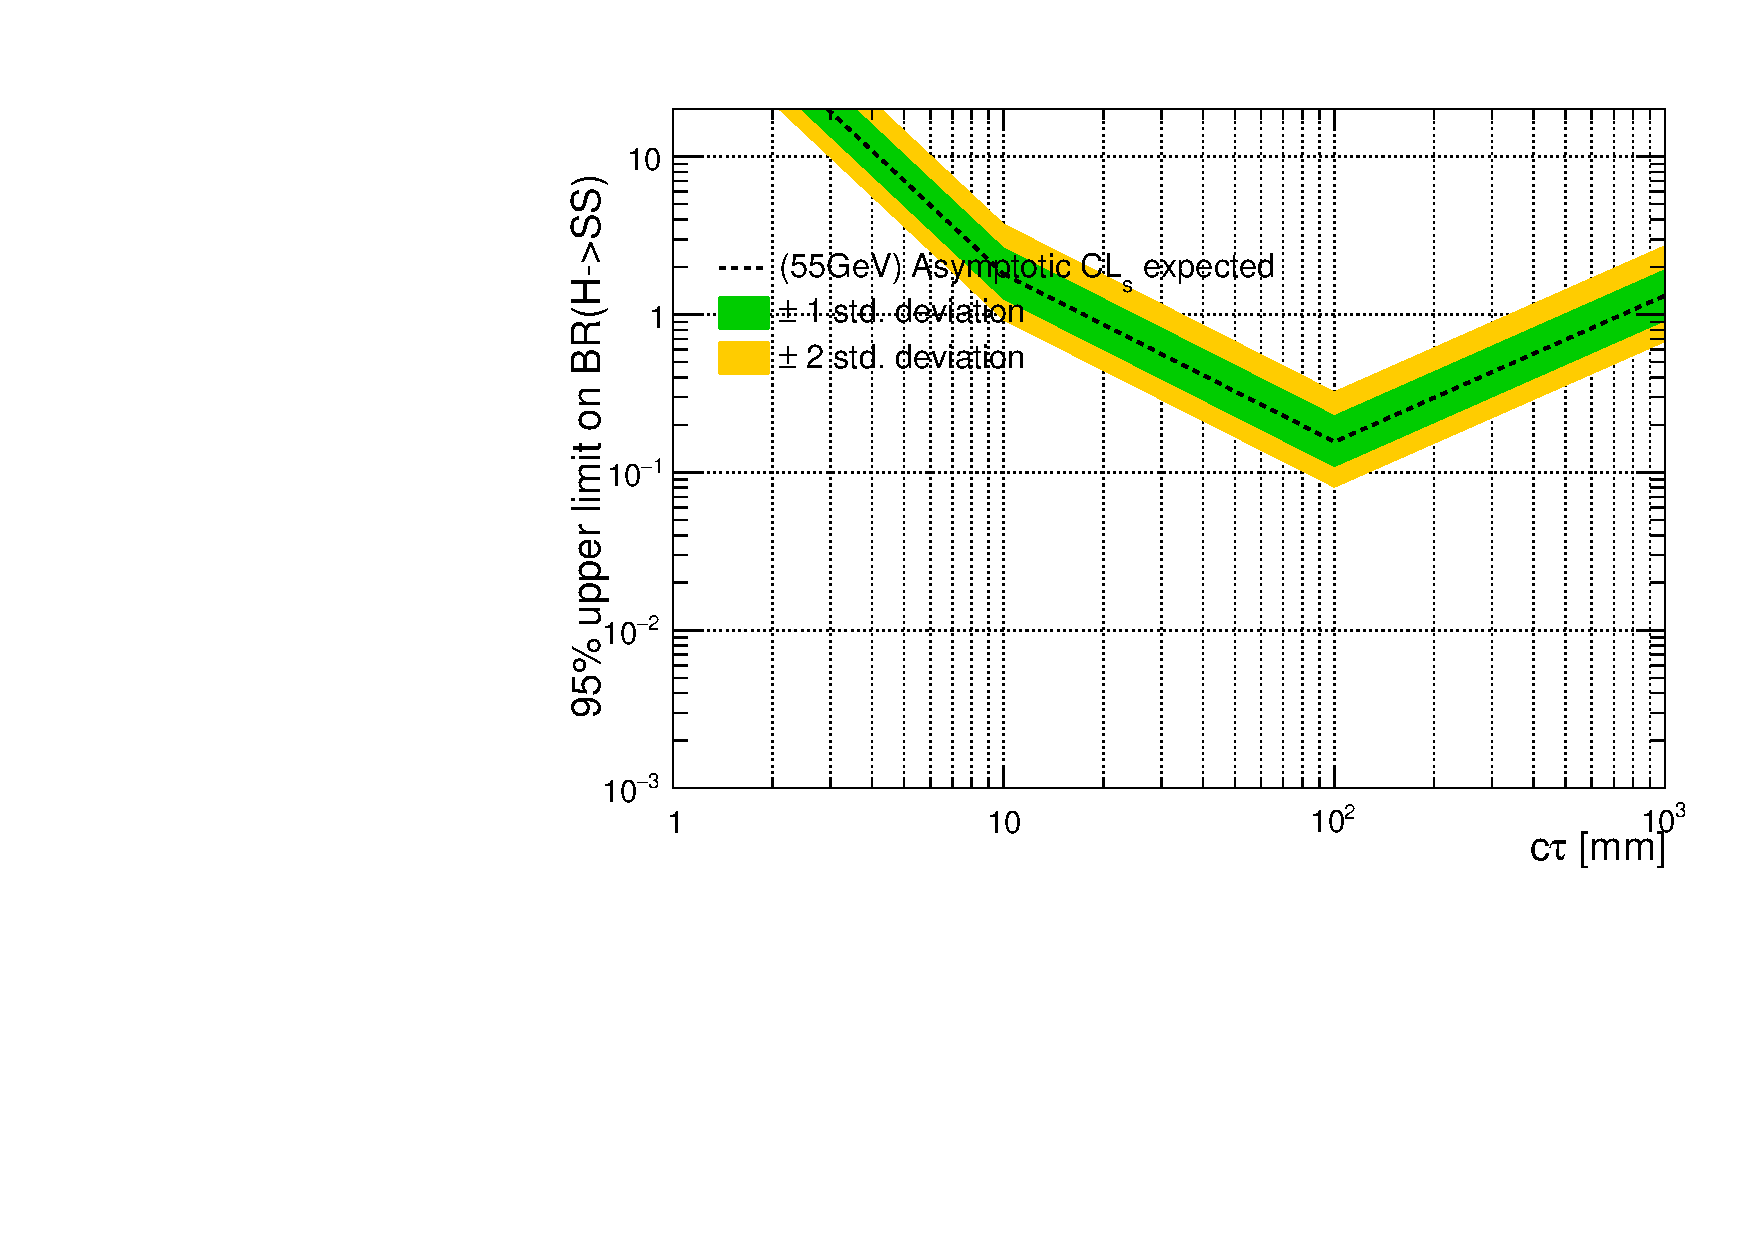
\includegraphics[width=0.48\linewidth]{figs/55GeVUpperLimit.pdf}
 \end{figure}
